\chapter{Conception}

%%%%%%%%%%%%%%%%%%%%%%%%%%%%% Introduction %%%%%%%%%%%%%%%%%%%%%%%%%%%%%

\section*{Introduction}

This chapter presents the design choices and reasoning behind the development of our Collaborative Highway Surveillance (CHS) system for detecting and responding to speeding violations in real time. It introduces the hybrid architecture combining UAVs and ground speed sensors, outlines the challenges related to communication latency, energy constraints, and coverage optimization, and explains the strategies applied to ensure reliable data exchange between all components.

We then describe the control logic of the system, which integrates a distributed drone selection algorithm based on residual energy and proximity, as well as a routing mechanism leveraging a hierarchical network of ground nodes to guide UAVs towards high-infraction zones. While this architecture ensures adaptability and responsiveness, the integration of prediction capabilities using machine learning introduces additional computational requirements that may challenge onboard resources.

To address this, we design a lightweight communication and decision-making protocol using MAVLink and UDP, enabling drones to exchange essential operational data efficiently while offloading heavy processing to ground stations when possible. Various simplification techniques and modular implementations are applied to balance decision accuracy with real-time performance and system scalability.

By combining robust communication, an adaptive control algorithm, and predictive analytics, the goal is to build a surveillance system that is both effective and deployable in real-world highway monitoring scenarios.

%%%%%%%%%%%%%%%%%%%%%%%%%%%%% Problematic and Objectives %%%%%%%%%%%%%%%%%%%%%%%%%%%%%

\section{Problematic and Objectives}
% Summarize limitations of existing systems, your specific goals, and constraints

\subsection*{Problematic}
Road safety remains a major public concern worldwide, with excessive speed being one of the leading causes of serious and fatal accidents. Conventional speed enforcement methods, such as fixed roadside radars, have shown limited effectiveness over time. Their locations are often publicly known and reported in real-time via mobile applications, allowing some drivers to slow down momentarily before the control point and accelerate again immediately afterwards. 

To address this limitation, certain high-risk road segments are occasionally monitored using helicopters. While effective in terms of detection, this method is costly in terms of human resources, fuel, and operational logistics, and it cannot ensure continuous large-scale coverage. As a result, many high-speed violation hotspots remain unmonitored, leaving a significant gap in traffic law enforcement.

Recent advances in Unmanned Aerial Vehicles (UAVs) have opened new perspectives for intelligent, mobile, and cost-effective traffic surveillance. UAVs can be rapidly deployed, repositioned in real time, and equipped with various sensors to monitor vehicle behavior. However, existing UAV-based solutions often rely on probabilistic flight plans without precise knowledge of the real-time distribution of traffic violations. Additionally, many approaches use UAVs in isolation, without integration into a larger, coordinated sensor network. This leads to inefficient coverage, redundant deployments, and higher energy consumption, ultimately reducing the operational lifespan of the system.

The core challenge, therefore, lies in designing a surveillance architecture that combines the mobility and flexibility of UAVs with the persistent monitoring capability of ground-based sensors. Such a system must intelligently detect high-risk zones, allocate UAV resources efficiently, and adapt dynamically to traffic conditions, all while operating within constraints of energy, communication range, and cost.

\subsection*{Objectives}
The main objective of this work is to design and validate a collaborative hybrid architecture for highway speed surveillance that significantly improves detection efficiency compared to existing fixed or isolated UAV systems.

The specific objectives are as follows:
\begin{itemize}
    \item \textbf{Develop a closed-loop collaborative surveillance system} (Collaborative Highway Surveillance – CHS) combining UAVs and wireless ground speed sensors for real-time detection and tracking of speeding vehicles.
    \item \textbf{Implement an efficient communication protocol} enabling UAV-to-UAV and UAV-to-ground data exchange, allowing the sharing of key information such as vehicle speed, UAV position, and residual energy levels.
    \item \textbf{Design a distributed decision-making algorithm} to select the most suitable UAV for deployment to detected infraction hotspots, based on criteria such as energy availability and distance.
    \item \textbf{Integrate an onboard computer vision module} to enable UAVs to autonomously identify and classify vehicles, providing visual confirmation of detected violations.
    \item \textbf{Introduce predictive surveillance capabilities} through Machine Learning algorithms trained on historical and real-time speed data, enabling early UAV deployment to anticipated violation zones.
    \item \textbf{Maximize coverage and operational lifespan} of the surveillance network through optimal task allocation, hierarchical sensor deployment, and adaptive routing strategies.
\end{itemize}

%%%%%%%%%%%%%%%%%%%%%%%%%%%%% Overview of the Proposed Solution %%%%%%%%%%%%%%%%%%%%%%%%%%%%%



\section{Overview of the Proposed Solution}

The proposed \textbf{Collaborative Highway Surveillance (CHS)} system aims to overcome the limitations of traditional speed enforcement methods by combining the adaptability of Unmanned Aerial Vehicles (UAVs) with the persistent monitoring capabilities of a ground-based sensor network. The system operates in a closed-loop fashion: speeding events are detected by ground sensors, which trigger the deployment of UAVs to the corresponding high-risk areas. 

Once on site, UAVs equipped with onboard cameras and computer vision modules can confirm violations in real time and transmit evidence to Mobile Base Stations (MBS) for enforcement. This hybrid approach ensures optimal coverage of the monitored road network, reduces redundant drone deployments, and improves energy efficiency. Furthermore, predictive analytics are incorporated to anticipate high-risk zones, enabling proactive rather than reactive surveillance. 

This section presents the conceptual operation of CHS, while the following \textit{System Architecture} subsection details the physical and logical organization of its components and their interactions.

\subsection{System Architecture}

The \textbf{CHS architecture} is designed as a multi-layered, hybrid network integrating aerial and ground-based elements to ensure continuous, adaptive, and efficient traffic surveillance. It is composed of the following main components:

\begin{itemize}
    \item \textbf{UAVs (Unmanned Aerial Vehicles)}: serve as the mobile aerial units of the system, capable of being dynamically deployed to specific locations as soon as a speeding event is detected. They are equipped with high-resolution cameras for capturing real-time video footage of vehicles, and onboard computing platforms such as Raspberry Pi or NVIDIA Jetson for running computer vision algorithms. These algorithms enable vehicle detection, tracking, and speed estimation directly on the UAV, reducing the need for constant ground-based processing. UAVs are also fitted with wireless communication modules to exchange data with ground nodes and Mobile Base Stations (MBS), and they can operate autonomously or semi-autonomously with automated path planning and obstacle avoidance.
    \item \textbf{RN (Reporting Nodes)}:  are fixed ground-based units positioned along monitored highways at regular intervals. Each RN is equipped with speed detection sensors such as radar, LIDAR, or magnetic sensors to monitor passing vehicles. When a vehicle exceeds the legal speed limit, the RN generates a violation alert that includes contextual data such as the timestamp, GPS position, and detected speed. This information is then transmitted to the nearest UAV or Helping Node (NH). Designed for continuous operation, RNs consume minimal energy to support long-term deployment in remote or infrastructure-limited locations.
    \item \textbf{NH (Helping Nodes)}: function as intermediate communication relays between RNs, UAVs, and MBS. Their primary role is to enable multi-hop wireless connectivity, extending the operational coverage area and maintaining communication in environments where direct line-of-sight is not possible. NH nodes also contribute to redundancy and fault tolerance by providing alternative data transmission paths in case of node failure or poor connectivity. These nodes can be mounted on existing roadside infrastructure such as lamp posts or integrated into mobile platforms for flexible placement.
    \item \textbf{MBS (Mobile Base Stations)}: are ground-based enforcement units, typically operated by traffic police or highway patrol officers. They receive validated infraction reports from UAVs, which include photographic evidence, GPS coordinates, and measured vehicle speed. Based on this information, MBS operators can initiate immediate enforcement actions such as dispatching officers, issuing electronic tickets, or recording violations in a centralized database. In addition to their enforcement role, MBS act as control hubs for UAV operations, managing mission assignments, receiving live video feeds, and storing collected evidence for later review.
\end{itemize}

% serve as the mobile aerial units of the system, capable of being dynamically deployed to specific locations as soon as a speeding event is detected. They are equipped with high-resolution cameras for capturing real-time video footage of vehicles, and onboard computing platforms such as Raspberry Pi or NVIDIA Jetson for running computer vision algorithms. These algorithms enable vehicle detection, tracking, and speed estimation directly on the UAV, reducing the need for constant ground-based processing. UAVs are also fitted with wireless communication modules to exchange data with ground nodes and Mobile Base Stations (MBS), and they can operate autonomously or semi-autonomously with automated path planning and obstacle avoidance.


The CHS system follows a closed-loop control process:
\begin{enumerate}[label=\arabic*., leftmargin=2em]
    \item \textbf{Detection Layer:} RN sensors monitor vehicle speeds and detect violations in real time.
    \item \textbf{Communication Layer:} NH nodes relay detection data to UAVs using a multi-hop wireless protocol.
    \item \textbf{Decision Layer:} UAVs exchange data and execute a distributed selection algorithm to assign the most suitable drone to each hotspot.
    \item \textbf{Action Layer:} The selected UAV navigates to the target area, visually confirms violations using onboard computer vision, and transmits evidence to the nearest MBS.
\end{enumerate}


% The CHS system follows a closed-loop control process:
% \begin{enumerate}
%     \item \textbf{Detection Layer:} RN sensors monitor vehicle speeds and detect violations in real time.
%     \item \textbf{Communication Layer:} NH nodes relay detection data to UAVs using a multi-hop wireless protocol.
%     \item \textbf{Decision Layer:} UAVs exchange data and execute a distributed selection algorithm to assign the most suitable drone to each hotspot.
%     \item \textbf{Action Layer:} The selected UAV navigates to the target area, visually confirms violations using onboard computer vision, and transmits evidence to the nearest MBS.
% \end{enumerate}

Figure~\ref{fig:chs_architecture} illustrates the overall architecture of the CHS system, showing the main components, data flows, and interactions between layers.

\begin{figure}[H]  
    \centering
    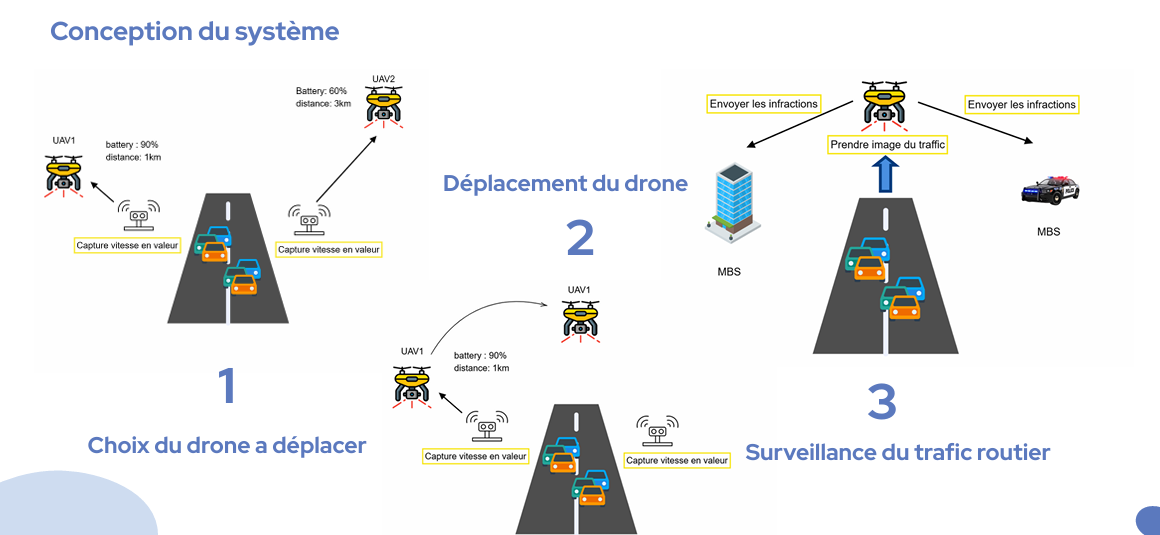
\includegraphics[width=1.0\textwidth]{Figures/Chapter4/Section2/archi.png} % Adjust width as needed
    \caption{Proposed CHS system architecture.}
    \label{fig:chs_architecture} % Reference label
\end{figure}

% \begin{figure}[H]  
%     \centering
%     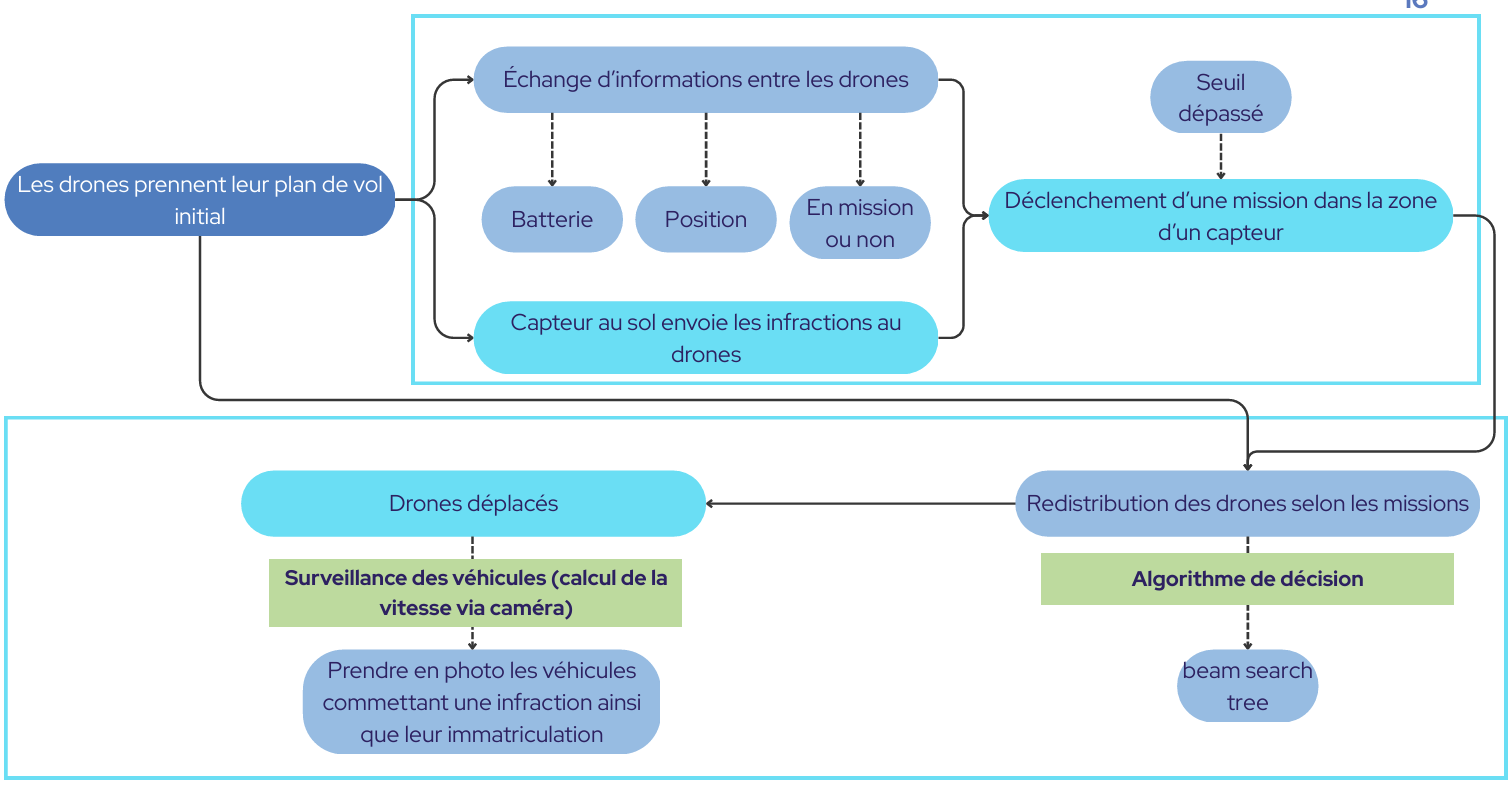
\includegraphics[width=1.0\textwidth]{Figures/Chapter4/Section2/diag.png} % Adjust width as needed
%     \caption{Proposed CHS system diag.}
%     \label{fig:chs_diag} % Reference label
% \end{figure}


% \subsection{Component Description}
% % Describe each main component of the system:
% %   - UAVs: roles, onboard modules, flight capabilities
% %   - RN (Reporting Nodes): ground speed sensors
% %   - NH (Helping Nodes): communication relays
% %   - MBS (Mobile Base Stations): mobile patrols

% The CHS system relies on the interaction of multiple specialized components. Each plays a crucial role in ensuring efficient and adaptive traffic surveillance.

% \begin{itemize}
%     \item \textbf{Unmanned Aerial Vehicles (UAVs):} These drones are equipped with high-resolution cameras, onboard processors, and communication modules. They perform the following tasks:
%     \begin{itemize}
%         \item Navigate autonomously to high-risk areas identified by ground sensors.
%         \item Detect and confirm speeding vehicles using computer vision algorithms.
%         \item Transmit violation data to Mobile Base Stations (MBS) for enforcement.
%         \item Monitor their own energy levels and coordinate with other UAVs to optimize coverage.
%     \end{itemize}

%     \item \textbf{Reporting Nodes (RN):} Ground-based sensors installed along highways. Their main functions are:
%     \begin{itemize}
%         \item Measure vehicle speeds and detect infractions in real time.
%         \item Send alerts and relevant data (e.g., speed, timestamp, location) to UAVs via multi-hop communication.
%         \item Provide data for predictive analytics to anticipate high-risk zones.
%     \end{itemize}

%     \item \textbf{Helping Nodes (NH):} These relay nodes enhance network connectivity:
%     \begin{itemize}
%         \item Act as communication bridges between RNs, UAVs, and MBS.
%         \item Ensure reliable data transfer even when direct communication links are unavailable.
%         \item Maintain network stability and reduce packet loss in areas with sparse coverage.
%     \end{itemize}

%     \item \textbf{Mobile Base Stations (MBS):} Ground patrol units responsible for enforcement:
%     \begin{itemize}
%         \item Receive verified infraction reports from UAVs.
%         \item Execute interventions on detected violations.
%         \item Maintain logs for traffic authorities and provide feedback to improve predictive models.
%     \end{itemize}
% \end{itemize}

% This detailed breakdown of each component clarifies their responsibilities and highlights the collaborative nature of the CHS system, ensuring real-time adaptive surveillance across the monitored highways.



\subsection{Communication Framework}

The efficiency of the CHS system relies heavily on a robust communication framework that ensures seamless data exchange between UAVs, ground sensors, and Mobile Base Stations (MBS). The framework is designed to be both real-time and resilient, adapting to dynamic traffic conditions and UAV movements.

\begin{itemize}
    \item \textbf{UAV-to-UAV Communication:}  
    UAVs exchange information about their current positions, battery levels, assigned patrol zones, and ongoing tasks to maintain a shared operational picture of the monitored highway network. This exchange supports the distributed decision-making algorithm, which selects the most suitable UAV to address new incidents or respond to emerging high-risk areas. To ensure interoperability and reliability, the MAVLink protocol is adopted, enabling standardized message formats and robust data delivery even under variable signal conditions. This communication channel is particularly important in multi-drone deployments, where coordination prevents redundant coverage and optimizes flight paths for energy efficiency.

    \item \textbf{UAV-to-Ground Sensors (RNs and NHs):}  
    Ground-based Reporting Nodes (RNs) act as the initial source of infraction data, detecting speeding vehicles and transmitting alerts that include speed measurements, timestamps, and GPS coordinates. These alerts are relayed to UAVs either directly or via intermediate Helping Nodes (NHs), which extend communication range through multi-hop routing. This mechanism ensures that UAVs maintain situational awareness even in areas with limited direct sensor coverage, allowing them to dynamically adjust their trajectories to intercept and verify violations in real time. By integrating both fixed and mobile communication elements, the system guarantees that UAVs receive timely and reliable updates regardless of terrain or infrastructure limitations.

    \item \textbf{UAV-to-Mobile Base Stations (MBS):}  
    Once a UAV has visually confirmed a traffic violation using its onboard computer vision system, it compiles a comprehensive evidence package that includes vehicle imagery or video, positional data, measured speed, and time of detection. This evidence is transmitted to the nearest MBS, where ground officers can initiate enforcement procedures such as issuing fines or intercepting the offending vehicle. Beyond enforcement, MBS units also serve as operational control points, providing UAVs with updated mission priorities, relaying new hotspot predictions, and adjusting patrol schedules based on the evolving traffic situation.

    \item \textbf{Data Management:}  
    To maintain operational integrity, all transmitted data is timestamped and geotagged, ensuring that every detected violation can be precisely traced to its origin. The framework prioritizes low-latency communication through the use of the UDP protocol, while incorporating error-checking mechanisms to mitigate packet loss or corruption. Collected datasets are stored in a structured format compatible with downstream processing by machine learning modules, enabling predictive analytics that identify recurring patterns, optimize UAV patrol strategies, and anticipate future violations. This approach ensures that communication not only supports immediate operational needs but also contributes to long-term system intelligence.
\end{itemize}

This communication framework enables collaborative, adaptive, and efficient surveillance, ensuring that each component of the CHS system can contribute effectively to reducing speeding violations across the monitored highway network.



% \subsection{Communication Framework}
% % Explain data exchanges:
% %   - Drone-to-drone
% %   - Drone-to-ground (RN/NH/MBS)
% %   - Routing strategies and multi-hop communication

% The efficiency of the CHS system relies heavily on a robust communication framework that ensures seamless data exchange between UAVs, ground sensors, and Mobile Base Stations (MBS). The framework is designed to be both real-time and resilient, adapting to dynamic traffic conditions and UAV movements.

% \begin{itemize}
%     \item \textbf{UAV-to-UAV Communication:} 
%     \begin{itemize}
%         \item UAVs share their current positions, energy levels, and assigned monitoring zones.
%         \item A distributed decision-making algorithm uses this data to coordinate which drone should move to a newly detected hotspot.
%         \item MAVLink protocol is used for reliable and standardized drone-to-drone messaging.
%     \end{itemize}

%     \item \textbf{UAV-to-Ground Sensors (RNs and NHs):} 
%     \begin{itemize}
%         \item Ground sensors transmit vehicle speed measurements and infractions to nearby UAVs.
%         \item Multi-hop routing through Helping Nodes ensures that UAVs receive real-time updates even in areas with sparse sensor coverage.
%         \item This communication allows UAVs to dynamically adapt flight paths to target high-risk zones.
%     \end{itemize}

%     \item \textbf{UAV-to-Mobile Base Stations (MBS):} 
%     \begin{itemize}
%         \item Once a UAV confirms a traffic violation, it sends detailed reports including vehicle position, speed, and captured images or video.
%         \item MBS units receive the data and initiate enforcement actions.
%         \item Feedback from MBSs can update UAV priorities and improve predictive models for future surveillance.
%     \end{itemize}

%     \item \textbf{Data Management:} 
%     \begin{itemize}
%         \item All exchanged information is timestamped and geotagged to ensure consistency and traceability.
%         \item UDP communication is used for low-latency data transmission, with error-checking mechanisms to handle packet loss.
%         \item The framework supports integration with machine learning modules for predictive analytics of traffic violations.
%     \end{itemize}
% \end{itemize}

% This communication framework enables collaborative, adaptive, and efficient surveillance, ensuring that each component of the CHS system can contribute to the overall goal of reducing speeding violations on monitored highways.



\subsection{Decision-Making and Control Logic}

The decision-making and control logic of the CHS system governs how UAVs respond to real-time traffic conditions and coordinate among themselves for optimal surveillance. This logic ensures that resources are efficiently allocated to high-risk zones while avoiding redundant coverage.

\begin{itemize}
    \item \textbf{Initial Patrol Planning:}  
    Before any mission is declared, each UAV follows a predefined initial patrol route designed to provide baseline coverage of the monitored highway network. These patrol paths are assigned to maximize spatial distribution and reduce the likelihood of coverage gaps. During this phase, UAVs operate autonomously, collecting environmental and traffic data while conserving energy through efficient path planning. This proactive patrolling ensures that the system maintains situational awareness even in the absence of active violations, and it positions UAVs strategically so that they can respond more rapidly when an infraction is detected.

    \item \textbf{Dynamic Zone Assignment:}  
    When a Reporting Node (RN) detects a speeding event, it sends a mission declaration to the network, specifying the location of the violation which directly corresponds to the sensor’s geographic position. At this moment, UAVs begin exchanging state information, including their current position, remaining battery level, and ongoing assignments. The distributed decision-making algorithm then evaluates which UAV is best suited to address the new mission based on proximity to the hotspot, energy reserves, and current workload. This ensures a quick and efficient allocation of resources, minimizing response time to high-risk areas.

    \item \textbf{Energy-Aware Routing:}  
    To maintain operational longevity, UAVs continually share battery status updates with nearby drones. The selection algorithm incorporates this information to ensure that only UAVs with sufficient energy are assigned to missions, avoiding situations where a drone might fail to complete its task due to battery depletion. This approach balances workload across the fleet, preventing overuse of individual UAVs and extending the system’s sustained surveillance capabilities.

    \item \textbf{Conflict Resolution:}  
    In scenarios where multiple UAVs are equally capable of responding to a mission, the system employs a conflict resolution strategy that prioritizes the UAV closest to the target zone while factoring in available energy. This prevents multiple UAVs from converging on the same hotspot unnecessarily, which reduces overlapping coverage and frees up other drones to remain on standby for future missions.

    \item \textbf{Adaptive Control Loops:}  
    The CHS operates in a continuous feedback loop, with UAVs, ground sensors, and Mobile Base Stations (MBS) exchanging operational data in real time. Insights from confirmed infractions, evolving traffic conditions, and predictive analytics allow the system to dynamically reassign UAVs, adjust flight paths, and update surveillance priorities. This adaptability ensures that UAV deployment is not only reactive to detected violations but also anticipates and prevents future incidents by focusing on areas with a high predicted risk.
\end{itemize}

This decision-making framework enables the CHS system to operate collaboratively, beginning with independent patrol patterns and transitioning into coordinated, data-driven missions when violations occur. As a result, the system maintains both proactive coverage and rapid, targeted responses to emerging threats.



% \subsection{Decision-Making and Control Logic}

% The decision-making and control logic of the CHS system governs how UAVs respond to real-time traffic conditions and coordinate among themselves for optimal surveillance. This logic ensures that resources are efficiently allocated to high-risk zones while avoiding redundant coverage.

% \begin{itemize}
%     \item \textbf{Dynamic Zone Assignment:}  
%     Each UAV continuously receives updated traffic information from the ground-based Reporting Nodes (RNs), including vehicle speed measurements and detected infractions. This incoming data is compared against predefined thresholds to identify potential hotspots, defined as zones where speeding frequency or severity exceeds normal levels. Once a hotspot is detected, a distributed decision-making algorithm evaluates all available UAVs to determine the most suitable one for deployment. This selection process accounts for the drone’s proximity to the target, its remaining battery capacity, and the current tasks assigned to other UAVs in the fleet. The result is a flexible allocation strategy that ensures rapid response to emerging incidents while maintaining balanced coverage across the monitored network.

%     \item \textbf{Energy-Aware Routing:}  
%     To maintain long-term operational effectiveness, UAVs regularly exchange information about their remaining battery levels with neighboring drones. The decision-making algorithm uses this information to prioritize drones that have sufficient energy to reach and monitor a target area without risking mission failure due to battery depletion. By considering both distance and energy reserves in task allocation, the system avoids assigning missions to UAVs that cannot be completed and prevents the overuse of individual units. This energy-aware approach not only extends the endurance of each mission but also contributes to the overall longevity of the UAV fleet.

%     \item \textbf{Conflict Resolution:}  
%     Situations may arise where multiple UAVs are suitable candidates for the same hotspot, potentially leading to redundant coverage and wasted resources. To address this, the system employs a conflict resolution mechanism that selects the UAV closest to the hotspot while also considering available energy reserves. By ensuring that only one UAV is dispatched per target zone, the system minimizes overlapping surveillance, reduces unnecessary energy expenditure, and allows other drones to remain available for new incidents. This prioritization process helps maintain high system responsiveness even when multiple events occur in quick succession.

%     \item \textbf{Adaptive Control Loops:}  
%     The CHS system operates within a continuous feedback loop where UAVs, ground sensors, and Mobile Base Stations (MBS) exchange operational data in real time. Feedback from confirmed infractions, evolving traffic conditions, and predictive models allows the system to dynamically reassign UAVs, modify flight paths, and update mission priorities. This adaptive control mechanism enables the CHS to respond proactively to emerging high-risk zones rather than simply reacting to detected violations. By continuously refining surveillance patterns based on the latest data, the system maintains a high level of efficiency and ensures that critical areas receive timely monitoring.
% \end{itemize}

% This decision-making framework allows the CHS system to operate collaboratively and intelligently, maximizing coverage of critical areas while conserving UAV energy and maintaining continuous surveillance.




% \subsection{Decision-Making and Control Logic}
% % Describe:
% %   - Hotspot detection (zones with high infractions)
% %   - Distributed selection algorithm (energy, distance)
% %   - Task allocation rules (avoiding multiple drones in same zone)

% The decision-making and control logic of the CHS system governs how UAVs respond to real-time traffic conditions and coordinate among themselves for optimal surveillance. This logic ensures that resources are efficiently allocated to high-risk zones while avoiding redundant coverage.

% \begin{itemize}
%     \item \textbf{Dynamic Zone Assignment:} 
%     \begin{itemize}
%         \item UAVs continuously receive data from Reporting Nodes (RNs) about vehicle speeds and infractions.
%         \item Each UAV compares received data with predefined thresholds to identify potential hotspots.
%         \item A distributed algorithm determines which UAV should move to a detected hotspot, considering distance, energy levels, and current assignments of other UAVs.
%     \end{itemize}

%     \item \textbf{Energy-Aware Routing:} 
%     \begin{itemize}
%         \item UAVs report their remaining battery levels to neighboring drones.
%         \item The algorithm prioritizes drones with sufficient energy to reach the target zone, avoiding situations where a UAV fails to complete its monitoring mission.
%         \item Energy-aware decisions also prevent overuse of individual UAVs, extending the operational lifetime of the fleet.
%     \end{itemize}

%     \item \textbf{Conflict Resolution:} 
%     \begin{itemize}
%         \item If multiple UAVs are candidates for the same hotspot, the system resolves conflicts by selecting the UAV closest to the zone with the highest remaining energy.
%         \item This ensures only one UAV is assigned per hotspot, reducing overlapping coverage and conserving resources.
%     \end{itemize}

%     \item \textbf{Adaptive Control Loops:} 
%     \begin{itemize}
%         \item Feedback from UAVs, ground sensors, and Mobile Base Stations (MBS) continuously adjusts flight paths and priorities.
%         \item The system dynamically reallocates UAVs in response to newly emerging traffic patterns or infractions.
%         \item This closed-loop control ensures that high-risk zones are monitored in real-time and that the overall system adapts efficiently to changing conditions.
%     \end{itemize}
% \end{itemize}

% This decision-making framework allows the CHS system to operate collaboratively and intelligently, maximizing coverage of critical areas while conserving UAV energy and maintaining continuous surveillance.







\subsection{Onboard Computer Vision Module for Vehicle Detection}

The CHS system integrates a sophisticated computer vision module on each UAV to detect and track vehicles in real time, calculate their speed, identify speeding violations, and signal the presence of such violations to the rest of the network. This module significantly enhances surveillance capabilities by enabling autonomous detection of speeding vehicles and supporting dynamic hotspot monitoring without relying solely on ground sensors.

\begin{itemize}
    \item \textbf{Camera Integration:}  
    Each UAV is equipped with a high-resolution camera capable of capturing continuous video streams in real time. The camera is mounted on a gimbal-stabilized platform to ensure sharp, clear imagery even during UAV movement, turbulence, or sudden maneuvers. This stabilization is essential for accurate detection, as motion blur or misalignment could compromise vehicle tracking and speed estimation. The optical system is also optimized for varying lighting conditions, enabling the UAV to operate effectively during both daytime and nighttime missions.

    \item \textbf{Vehicle Detection Algorithm:}  
    The onboard processing unit runs advanced machine learning-based object detection algorithms, such as YOLO (You Only Look Once), to identify vehicles within the video frames. This detection process involves both localization drawing bounding boxes around detected objects and classification, differentiating between various types of vehicles such as cars, trucks, and motorcycles. This classification capability not only aids in identifying specific offenders but also provides valuable traffic composition data for further analysis and prediction.

    \item \textbf{Speed Estimation:}  
    Once vehicles are detected, the system tracks their positions across consecutive frames using multi-object tracking techniques. By combining this positional data with UAV telemetry, including altitude, GPS location, and camera angle, the system accurately calculates the speed of each vehicle. Vehicles that exceed a predefined speed threshold are immediately flagged as violations. This automated approach eliminates the need for manual intervention and ensures that even brief violations are captured.

    \item \textbf{Data Transmission:}  
    When a violation is confirmed, the UAV compiles a detailed report that includes the vehicle type, geographic position, calculated speed, and supporting visual evidence such as images or short video clips. This data is transmitted in near real time to the Mobile Base Stations (MBS) through the CHS communication framework. The rapid delivery of this information enables ground enforcement teams to act quickly, whether by intercepting the vehicle or logging the infraction for later penalties.

    \item \textbf{Integration with Decision-Making:}  
    The outputs of the computer vision module are directly integrated into the UAV’s decision-making logic. Detection results influence the prioritization of surveillance zones, allowing UAVs to dynamically adjust their flight paths toward areas with higher observed violation rates. This real-time feedback loop ensures that UAVs focus on locations where their presence will have the greatest impact, thereby increasing the overall effectiveness and efficiency of the CHS system in mitigating speeding incidents.
\end{itemize}

The onboard computer vision module transforms each UAV into an intelligent, autonomous monitoring unit capable of independently detecting, verifying, and reporting traffic violations. By combining high-quality imaging, advanced object recognition, precise speed estimation, and seamless integration with the decision-making framework, this module plays a pivotal role in achieving continuous and targeted highway surveillance.



\subsection{Predictive Surveillance Module}

In the current CHS architecture, there exists a limitation: when a vehicle triggers a mission by being detected speeding by a ground sensor, it may already be too late to capture visual evidence, as the sensor itself lacks a camera and the offending vehicle might have already left the monitored zone. The Predictive Surveillance Module addresses this challenge by enabling proactive UAV positioning before the arrival of a potential violator. By leveraging historical data, real-time measurements, and machine learning techniques, the module forecasts where infractions are most likely to occur, thereby reducing UAV response time and increasing capture rates.

\begin{itemize}
    \item \textbf{Data Sources:}  
    The predictive module aggregates information from multiple sources to build a comprehensive traffic behavior profile. Historical traffic data, collected from Reporting Nodes (RNs) and past UAV mission records, form the foundation for long-term pattern analysis. Public datasets, such as those available from \textit{data.gouv.fr} in France, are also integrated to enrich the historical database with broader traffic trends. In addition, real-time inputs such as current speed measurements from RNs, infraction reports from UAVs, and enforcement data from Mobile Base Stations (MBS) ensure that the predictive model remains aligned with current conditions.

    \item \textbf{Machine Learning Algorithms:}  
    The module employs advanced supervised learning models, including Random Forests, Gradient Boosting Machines, and Neural Networks, to identify patterns associated with speeding or hazardous driving. These models are trained on labeled datasets containing both historical and real-time features, such as traffic density, time of day, and weather conditions. The algorithms process this data to produce probabilistic forecasts of speeding incidents for different road segments, enabling the CHS system to move beyond purely reactive surveillance.

    \item \textbf{Hotspot Prediction:}  
    The predictive engine continuously updates a dynamic map of high-risk zones, recalculating probabilities as fresh sensor and UAV data arrives. When a particular segment shows an elevated likelihood of violation, it is flagged as a predicted hotspot. This allows UAVs to be dispatched to these locations ahead of time, increasing the probability of capturing a violation as it occurs rather than after the fact. This capability is especially useful in rural or sparsely monitored areas where ground sensors are widely spaced.

    \item \textbf{Integration with UAV Decision-Making:}  
    Predictions generated by the module are directly fed into the UAV decision-making and control logic. This ensures that the system’s routing and scheduling algorithms can proactively allocate UAVs to areas of concern before a violation is even detected. In doing so, the predictive component complements the reactive monitoring provided by the onboard vision system, creating a hybrid strategy that combines foresight with immediate situational awareness.

    \item \textbf{Performance Feedback:}  
    To maintain and improve accuracy over time, the module incorporates a continuous learning loop. After each mission, predicted infractions are compared against actual detections to evaluate model performance. Discrepancies between prediction and reality are analyzed and used to retrain the models, enabling gradual refinement. This adaptive learning approach ensures that the predictive module becomes increasingly reliable, ultimately leading to smarter UAV deployment and more efficient highway surveillance.
\end{itemize}

By anticipating potential violations rather than merely responding to them, the Predictive Surveillance Module transforms the CHS system into a proactive enforcement tool. This not only improves the capture rate of speeding vehicles but also allows for more strategic use of UAV resources, maximizing coverage and minimizing wasted flight time.




% \subsection{Predictive Surveillance Module}
% % Data collection/preprocessing from RN or public datasets
% % ML model for early prediction of infractions
% % How predictions integrate into CHS for proactive drone deployment


% The Predictive Surveillance Module enhances the CHS system by forecasting potential traffic infractions and enabling proactive UAV deployment. This module uses historical and real-time data to predict hotspots, improving coverage and reducing response time.

% \begin{itemize}
%     \item \textbf{Data Sources:} 
%     \begin{itemize}
%         \item Historical traffic data from ground sensors (Reporting Nodes) and past UAV missions.
%         \item Real-time speed measurements and incident reports transmitted by UAVs and Mobile Base Stations (MBS).
%     \end{itemize}

%     \item \textbf{Machine Learning Algorithms:} 
%     \begin{itemize}
%         \item Supervised learning models (e.g., Random Forest, Gradient Boosting, or Neural Networks) are trained to identify patterns leading to speeding or risky driving behavior.
%         \item The models output probabilities for potential infractions across different road segments.
%     \end{itemize}

%     \item \textbf{Hotspot Prediction:} 
%     \begin{itemize}
%         \item Predicted high-risk zones are continuously updated as new data arrives.
%         \item UAVs receive prioritized task assignments based on these predictions, allowing for early monitoring of likely violation points.
%     \end{itemize}

%     \item \textbf{Integration with UAV Decision-Making:} 
%     \begin{itemize}
%         \item Predicted hotspots feed directly into the decision-making and control logic, guiding UAV routing and scheduling.
%         \item This proactive approach complements reactive monitoring from the onboard vision module, ensuring comprehensive surveillance.
%     \end{itemize}

%     \item \textbf{Performance Feedback:} 
%     \begin{itemize}
%         \item The system compares predicted infractions with actual detections, refining the prediction models over time.
%         \item Continuous learning ensures improved accuracy and efficiency in UAV deployment.
%     \end{itemize}
% \end{itemize}

% By predicting potential infractions, the Predictive Surveillance Module enables the CHS system to anticipate traffic violations, optimize UAV deployment, and maximize overall surveillance effectiveness.



%%%%%%%%%%%%%%%%%%%%%%%%%%%%% Conclusion %%%%%%%%%%%%%%%%%%%%%%%%%%%%%



\section{Conclusion}
% Recap of the proposed architecture
% Prepare transition into the Implementation chapter

In this chapter, we have presented the design of the Collaborative Highway Surveillance (CHS) system, detailing its architecture, components, and functional modules. The system combines UAVs, ground sensors, and mobile base stations to achieve real-time, adaptive monitoring of highway traffic. Key aspects include:

\begin{itemize}
    \item A \textbf{modular architecture} that ensures scalability, fault tolerance, and efficient integration of UAVs and ground sensors.
    \item A \textbf{communication framework} enabling reliable data exchange between UAVs, ground nodes, and mobile base stations.
    \item A \textbf{decision-making and control logic} that dynamically allocates UAVs to high-risk zones based on energy levels, distance, and real-time traffic conditions.
    \item An \textbf{onboard computer vision module} that detects and tracks vehicles in real-time, supporting automatic identification of traffic violations.
    \item A \textbf{predictive surveillance module} that leverages machine learning to anticipate infractions, guiding UAVs proactively to potential hotspots.
\end{itemize}

Overall, the proposed solution provides a comprehensive and intelligent approach to highway surveillance, enhancing the efficiency of traffic monitoring while reducing the reliance on costly human-operated interventions. This chapter lays the foundation for the next chapter, which focuses on the implementation and experimental evaluation of the CHS system.